


\tikzset{every picture/.style={line width=0.75pt}} %set default line width to 0.75pt        

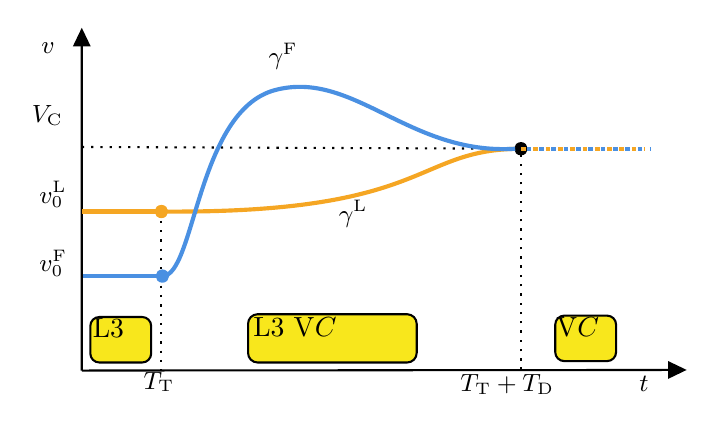
\begin{tikzpicture}[x=0.75pt,y=0.75pt,yscale=-1,xscale=1]
%uncomment if require: \path (0,300); %set diagram left start at 0, and has height of 300

%Straight Lines [id:da35056627418722197] 
\draw    (40.89,169.47) -- (329.33,169.18) ;
\draw [shift={(332.33,169.18)}, rotate = 179.94] [fill={rgb, 255:red, 0; green, 0; blue, 0 }  ][line width=0.08]  [draw opacity=0] (8.93,-4.29) -- (0,0) -- (8.93,4.29) -- cycle    ;
%Straight Lines [id:da28683350838432653] 
\draw    (40.89,169.47) -- (40.9,7.33) ;
\draw [shift={(40.9,4.33)}, rotate = 90] [fill={rgb, 255:red, 0; green, 0; blue, 0 }  ][line width=0.08]  [draw opacity=0] (8.93,-4.29) -- (0,0) -- (8.93,4.29) -- cycle    ;
%Curve Lines [id:da2653386554142514] 
\draw [color={rgb, 255:red, 245; green, 166; blue, 35 }  ,draw opacity=1 ][line width=1.5]    (79.26,92.86) .. controls (209.64,93.94) and (200.42,62.83) .. (252.48,62.61) ;
%Straight Lines [id:da3478445904699752] 
\draw [color={rgb, 255:red, 245; green, 166; blue, 35 }  ,draw opacity=1 ][line width=1.5]    (40.89,92.86) -- (79.26,92.86) ;
%Straight Lines [id:da4896997718287308] 
\draw [color={rgb, 255:red, 74; green, 144; blue, 226 }  ,draw opacity=1 ][line width=1.5]    (41.37,123.96) -- (76.96,123.96) ;
%Straight Lines [id:da9574639568141294] 
\draw  [dash pattern={on 0.84pt off 2.51pt}]  (40.88,61.75) -- (252.48,62.61) ;
%Straight Lines [id:da30746319484426654] 
\draw  [dash pattern={on 0.84pt off 2.51pt}]  (79.26,92.86) -- (79.26,169.54) ;
%Shape: Ellipse [id:dp4407398973997718] 
\draw  [color={rgb, 255:red, 245; green, 166; blue, 35 }  ,draw opacity=1 ][fill={rgb, 255:red, 245; green, 166; blue, 35 }  ,fill opacity=1 ] (76.5,92.86) .. controls (76.5,91.37) and (77.74,90.16) .. (79.26,90.16) .. controls (80.79,90.16) and (82.03,91.37) .. (82.03,92.86) .. controls (82.03,94.35) and (80.79,95.56) .. (79.26,95.56) .. controls (77.74,95.56) and (76.5,94.35) .. (76.5,92.86) -- cycle ;
%Shape: Ellipse [id:dp2316202221311856] 
\draw  [color={rgb, 255:red, 74; green, 144; blue, 226 }  ,draw opacity=1 ][fill={rgb, 255:red, 74; green, 144; blue, 226 }  ,fill opacity=1 ] (76.96,123.96) .. controls (76.96,122.47) and (78.2,121.26) .. (79.73,121.26) .. controls (81.25,121.26) and (82.49,122.47) .. (82.49,123.96) .. controls (82.49,125.45) and (81.25,126.66) .. (79.73,126.66) .. controls (78.2,126.66) and (76.96,125.45) .. (76.96,123.96) -- cycle ;
%Shape: Ellipse [id:dp3997364126281657] 
\draw  [color={rgb, 255:red, 0; green, 0; blue, 0 }  ,draw opacity=1 ][fill={rgb, 255:red, 0; green, 0; blue, 0 }  ,fill opacity=1 ] (249.72,62.61) .. controls (249.72,61.12) and (250.95,59.91) .. (252.48,59.91) .. controls (254.01,59.91) and (255.25,61.12) .. (255.25,62.61) .. controls (255.25,64.11) and (254.01,65.31) .. (252.48,65.31) .. controls (250.95,65.31) and (249.72,64.11) .. (249.72,62.61) -- cycle ;
%Straight Lines [id:da3200218142779261] 
\draw  [dash pattern={on 0.84pt off 2.51pt}]  (252.48,169.11) -- (252.48,62.61) ;
%Curve Lines [id:da37549686511164215] 
\draw [color={rgb, 255:red, 74; green, 144; blue, 226 }  ,draw opacity=1 ][line width=1.5]    (79.73,123.96) .. controls (95.44,124.26) and (96.31,44.25) .. (134.09,34.32) .. controls (171.86,24.38) and (198.58,65.85) .. (249.72,62.61) ;
%Straight Lines [id:da07614497882926097] 
\draw [color={rgb, 255:red, 245; green, 166; blue, 35 }  ,draw opacity=1 ][line width=1.5]  [dash pattern={on 1.69pt off 2.76pt}]  (252.48,62.61) -- (311.91,62.61) ;
%Rounded Rect [id:dp019414369875309534] 
\draw  [color={rgb, 255:red, 0; green, 0; blue, 0 }  ,draw opacity=1 ][fill={rgb, 255:red, 248; green, 231; blue, 28 }  ,fill opacity=1 ] (45,148.05) .. controls (45,145.63) and (46.96,143.67) .. (49.39,143.67) -- (69.95,143.67) .. controls (72.37,143.67) and (74.33,145.63) .. (74.33,148.05) -- (74.33,161.21) .. controls (74.33,163.63) and (72.37,165.6) .. (69.95,165.6) -- (49.39,165.6) .. controls (46.96,165.6) and (45,163.63) .. (45,161.21) -- cycle ;
%Rounded Rect [id:dp5170385073800969] 
\draw  [color={rgb, 255:red, 0; green, 0; blue, 0 }  ,draw opacity=1 ][fill={rgb, 255:red, 248; green, 231; blue, 28 }  ,fill opacity=1 ] (121,146.99) .. controls (121,144.42) and (123.08,142.33) .. (125.65,142.33) -- (197.61,142.33) .. controls (200.18,142.33) and (202.27,144.42) .. (202.27,146.99) -- (202.27,160.94) .. controls (202.27,163.51) and (200.18,165.6) .. (197.61,165.6) -- (125.65,165.6) .. controls (123.08,165.6) and (121,163.51) .. (121,160.94) -- cycle ;
%Straight Lines [id:da23131458085088186] 
\draw [color={rgb, 255:red, 74; green, 144; blue, 226 }  ,draw opacity=1 ][line width=1.5]  [dash pattern={on 1.69pt off 2.76pt}]  (255.25,62.61) -- (314.67,62.61) ;
%Rounded Rect [id:dp9239181341405276] 
\draw  [color={rgb, 255:red, 0; green, 0; blue, 0 }  ,draw opacity=1 ][fill={rgb, 255:red, 248; green, 231; blue, 28 }  ,fill opacity=1 ] (269,147.39) .. controls (269,144.96) and (270.96,143) .. (273.39,143) -- (293.95,143) .. controls (296.37,143) and (298.33,144.96) .. (298.33,147.39) -- (298.33,160.54) .. controls (298.33,162.97) and (296.37,164.93) .. (293.95,164.93) -- (273.39,164.93) .. controls (270.96,164.93) and (269,162.97) .. (269,160.54) -- cycle ;

% Text Node
\draw (19.92,10) node [anchor=north west][inner sep=0.75pt]  [font=\small]  {$v$};
% Text Node
\draw (308.04,170.59) node [anchor=north west][inner sep=0.75pt]  [font=\small]  {$t$};
% Text Node
\draw (18.95,76.9) node [anchor=north west][inner sep=0.75pt]  [font=\small]  {$v_{0}^{\mathrm{L}}$};
% Text Node
\draw (18.95,109.73) node [anchor=north west][inner sep=0.75pt]  [font=\small]  {$v_{0}^{\mathrm{F}}$};
% Text Node
\draw (69.15,168.69) node [anchor=north west][inner sep=0.75pt]  [font=\small]  {$T_{\mathrm{T}}$};
% Text Node
\draw (129.41,10.14) node [anchor=north west][inner sep=0.75pt]  [font=\small]  {$\gamma ^{\mathrm{F}}$};
% Text Node
\draw (163.24,85.9) node [anchor=north west][inner sep=0.75pt]  [font=\small]  {$\gamma ^{\mathrm{L}}$};
% Text Node
\draw (15.33,40.32) node [anchor=north west][inner sep=0.75pt]  [font=\small]  {$V_{\mathrm{C}}$};
% Text Node
\draw (221.81,170.03) node [anchor=north west][inner sep=0.75pt]  [font=\small]  {$T_{\mathrm{T}} +T_{\mathrm{D}}$};
% Text Node
\draw (44.72,143) node [anchor=north west][inner sep=0.75pt]    {$\mathrm{L} 3$};
% Text Node
\draw (122.05,142.33) node [anchor=north west][inner sep=0.75pt]    {$\mathrm{L} 3\ \leftrightarrows \mathrm{V} C$};
% Text Node
\draw (268.05,142.33) node [anchor=north west][inner sep=0.75pt]    {$\mathrm{V} C$};


\end{tikzpicture}